%
% subsystems.tex
%
% Copyright (C) 2021 by SpaceLab.
%
% GOLDS-UFSC Documentation
%
% This work is licensed under the Creative Commons Attribution-ShareAlike 4.0
% International License. To view a copy of this license,
% visit http://creativecommons.org/licenses/by-sa/4.0/.
%

%
% \brief Subsystems chapter.
%
% \author Gabriel Mariano Marcelino <gabriel.mm8@gmail.com>
%
% \institution Universidade Federal de Santa Catarina (UFSC)
%
% \version 0.1.0
%
% \date 2020/06/06
%

\chapter{Subsystems} \label{ch:subsystems}

\begin{figure}[!ht]
    \begin{center}
        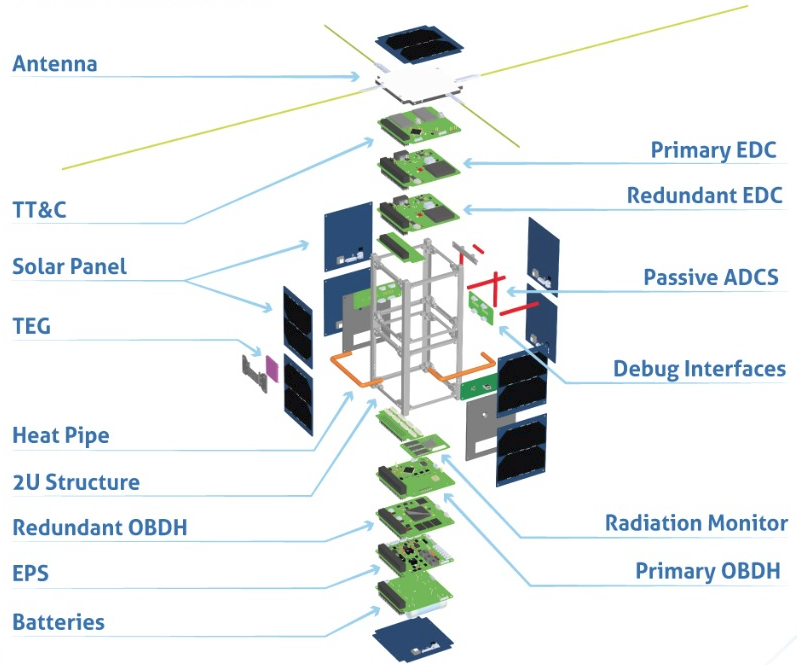
\includegraphics[width=\textwidth]{figures/exploded-view}
        \caption{Exploded view of the GOLDS-UFSC satellite.}
        \label{fig:exploded-view}
    \end{center}
\end{figure}

\section{On-Board Data Handling}

OBDH\nomenclature{\textbf{OBDH}}{\textit{On-Board Data Handling}.} \cite{obdh2}

\section{Telemetry, Tracking and Command Module}

TTC\nomenclature{\textbf{TTC}}{\textit{Telemetry, Tracking and Command Module}.} \cite{ttc}

\subsection{Antenna Module}

The used antenna module is the CubeSat deployable VHF and UHF antenna from ISISpace \cite{isis-antenna}. It is a four monopole antenna built with tape strings (up to 55 cm) and compliant with the CubeSat standard (dipole or turnstile options are also available). The deployment method is the burning wire and it can be controlled digitally through a I$^{2}$C interface. To allow redundancy, there are two independent deployment controllers that can be activated separately. Also, the construction of this module allows the installation of a solar panel at the top side. The RF gain is about 0 dBi.

A picture of the antenna module (with all antennas released) can be seen in \autoref{fig:isis-antenna}.

\begin{figure}[!ht]
    \begin{center}
        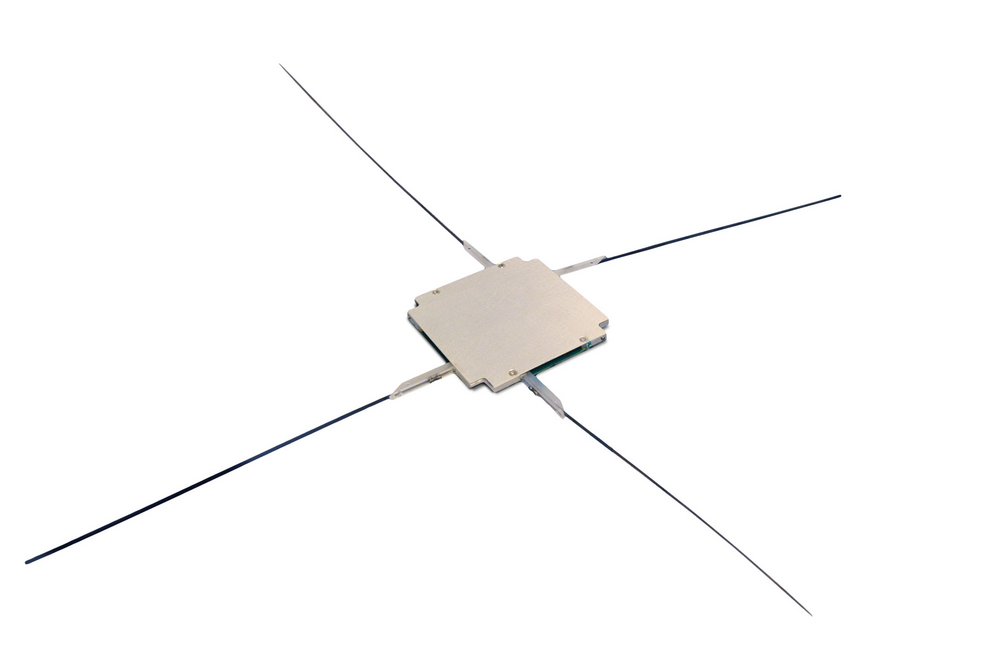
\includegraphics[width=0.8\textwidth]{figures/isis-antenna}
        \caption{Antenna module from ISISpace.}
        \label{fig:isis-antenna}
    \end{center}
\end{figure}

The chosen configuration for this mission can be seen below (using \autoref{fig:isis-antenna-ref} as reference):

\begin{itemize}
    \item Configuration: 4 monopoles (1x VHF + 3x UHF)
        \begin{itemize}
            \item Antenna 1: VHF - 145,97 MHz (beacon)
            \item Antenna 2: UHF - 401,635 MHz (EDC)
            \item Antenna 3: UHF - 436,9 MHz (downlink/uplink)
            \item Antenna 4: UHF - 401,635 MHz (redundant EDC)
        \end{itemize}
    \item Tuning structure size: 2U
    \item Mounting position: Top
    \item Supply voltage: 3,3 V
    \item I$^{2}$C control type: Dual bus
        \begin{itemize}
            \item Primary I$^{2}$C address: 31h (7-bit address)
            \item Redundant I$^{2}$C address: 32h (7-bit address)
        \end{itemize}
    \item I$^{2}$C watchdog: Enabled with a time out of 60 seconds.
\end{itemize}

\begin{figure}[!ht]
    \begin{center}
        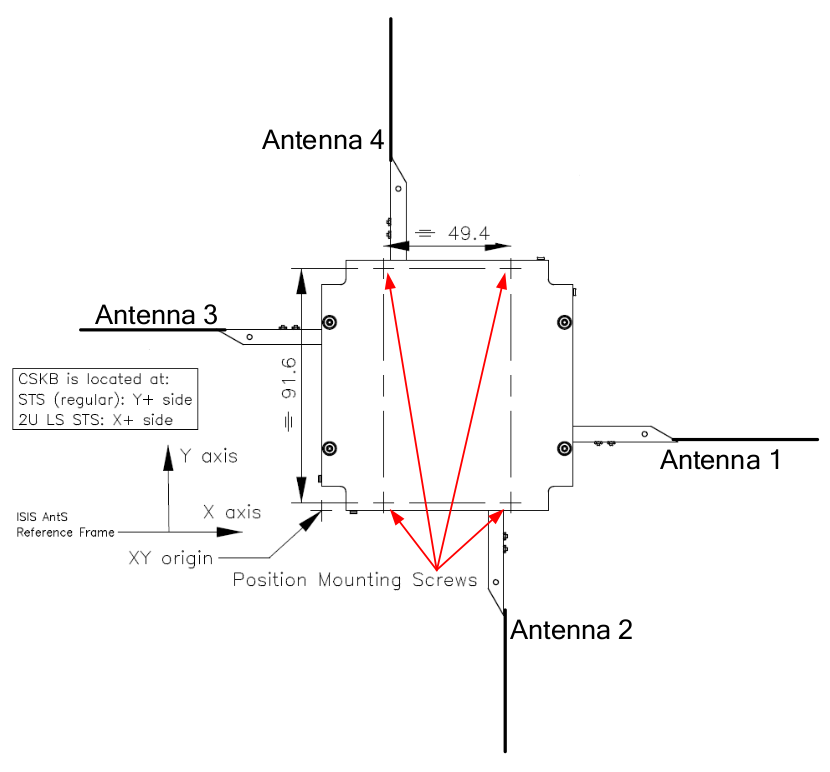
\includegraphics[width=0.7\textwidth]{figures/isis-antenna-ref}
        \caption{Configuration reference of the antenna module.}
        \label{fig:isis-antenna-ref}
    \end{center}
\end{figure}

In the digital interface, a temperature sensor and the state of four deployment switches (1 per monopole) are also available. These switches indicate if a monopole is released or not, and can be used as feedback of the deployment process.

\section{Electrical Power System}

EPS\nomenclature{\textbf{EPS}}{\textit{Electrical Power System}.} \cite{eps2}

\subsection{Battery Module}

\cite{bat4c}

\subsection{Solar Panels}

.

\subsection{Kill-Switches and RBF}

.

\section{Attitude Control System}

The Attitude Control System (ACS\nomenclature{\textbf{ACS}}{\textit{Attitude Control System}.}) is a passive attitude control system, which depends on the Earth's magnetic field to rotate and stabilize the satellite \cite{santoni2009,gerhardt2010}. The system is composed of one permanent magnet to create a force to align the magnet with the Earth's magnetic field and four hysteresis bars to damp the cube oscillations and achieve stabilization.

When equilibrium is achieved, the permanent magnet aligns itself to the Earth's field lines. The hysteresis bars convert oscillation and rotation energy into heat, maintaining the alignment through magnetic moment. The components are placed in positions as to minimize the magnet's interaction with the hysteresis bars, which limits the magnetic moment of the magnet \cite{francois2010}. \autoref{fig:adcs} shows the mounting of the hysteresis bars (green) and the permanent magnet (red) on the mechanical structure. The whole passive ACS was implemented according to \cite{francois2010}.

\begin{figure}[!ht]
    \begin{center}
        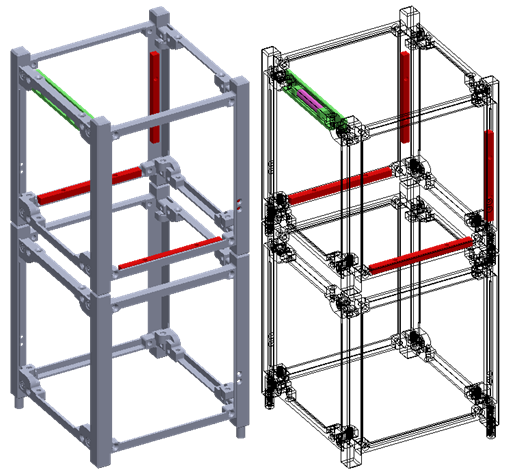
\includegraphics[width=0.7\textwidth]{figures/adcs}
        \caption{ACS subsytem. Rare earth magnet (pink) and hysteresis bars (red) installed in the structure.}
        \label{fig:adcs}
    \end{center}
\end{figure}

As a passive magnetic attitude control system is used, it is possible to stabilize only one axis, and so, the CubeSat will still slowly (due to hysteresis bars) rotate around this axis, even after stabilized. A N45 neodymium magnet and 4 hysteresis bars of Permanorm 5000 H2 are used (courtesy of Vacuumschmelze GmbH \& Co. KG). The material of the hysteresis bar is shaped in order to maximize the stabilization, which is the most important part of the attitude control.

Many conditions impact on the detumbling time, which is the time required for the satellite to stabilize. Magnetic passive attitude stabilization systems such as the one developed for this mission achieve the equilibrium state within a few weeks of operation \cite{santoni2009}.

The GOLDS-UFSC satellite does not feature an orbit control subsystem.

\section{Mechanical Structure}

.

\section{Interconnection Modules}

\subsection{PC-104 Interconnection Boards}

The PC-104 interconnection boards are intended to be used as an interconnection of the two PC-104 bus segments of the 2U structure (top and bottom units). This interconnection is made with a set of PicoBlade cables between the top and bottom boards. The set of two boards can be seen in \autoref{fig:pc104-adapter}.

\begin{figure}[!ht]
    \begin{center}
        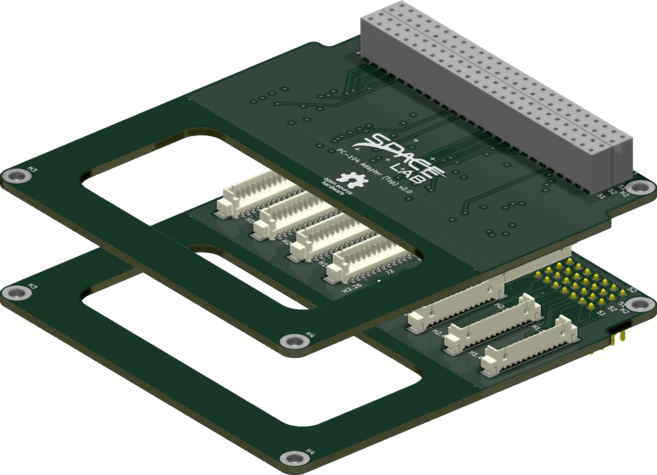
\includegraphics[width=0.7\textwidth]{figures/pc104-adapter}
        \caption{PC-104 adapter boards (top and bottom).}
        \label{fig:pc104-adapter}
    \end{center}
\end{figure}

More information about these boards can be found in \cite{pc104-boards}.

\subsection{External Connection Boards}

The Interstage Interface Panels (IIP) are three vertical internally mounted PCBs designed to give external access up to four modules inside of a 2U CubeSat during final assembly, integration and testing (AIT) before launch. The complete set of the boards allow the nanosatellite to be charged, programed and debugged. The usage of this hardware platform is taking into account the use of a MSP-FET: MSP430 Flash Emulation Tool from Texas Instruments for JTAG programing and debugging, UART debugging through a mini USB type B port interfacing the FT4232H USB bridge IC from FTDI, a JST XH header for charging internal batteries and a Remove Before Flight (RBF) pin header. The boards can seen in \autoref{fig:iip-boards}.

\begin{figure}[!ht]
    \begin{center}
        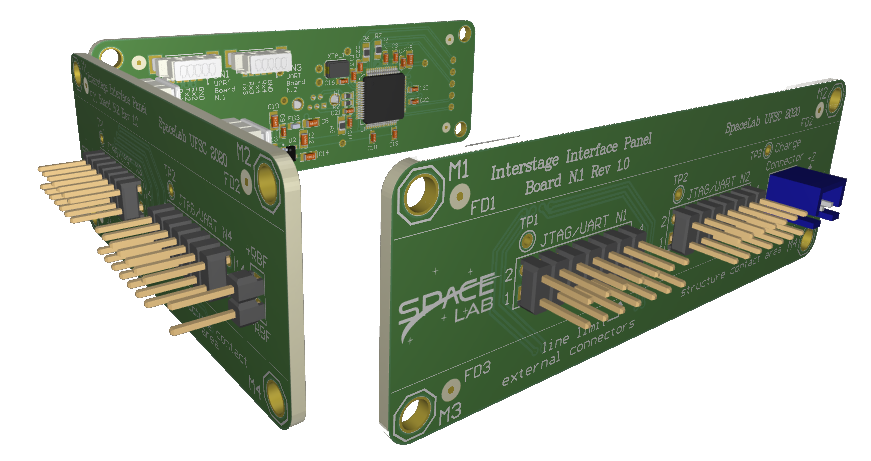
\includegraphics[width=0.7\textwidth]{figures/iip_fullset}
        \caption{Set of external connection boards.}
        \label{fig:iip-boards}
    \end{center}
\end{figure}

More information about these boards can be found in \cite{iip}.

\section{Payloads}

\subsection{Environmental Data Collection}

EDC\nomenclature{\textbf{EDC}}{\textit{Environmental Data Collection}.} \cite{edc}

\subsection{Redundant OBDH (Payload-X)}

Payload-x \cite{payload-x}

\subsection{Radiation Monitor}

.
